\section {Introduction\\}
Traditionally, the web server is a classical example of the request/response 
model, where the clients can retrieve the resource from the server, but the 
server cannot push the data to the client actively. 

However, with the increasing popularity of Ajax\cite{Ajax} technologies, there 
are many scenarios where servers would like to actively notify the clients the 
latest events. For example, the chat room, twitter timeline, stock ticker, etc.

To overcome the limitation of request/response model, many approaches has been 
proposed to build a more responsive site:

\begin{itemize}
\item Client Pull: the client pull approach is very easy to implement because 
it is stateless and the web server doesn't need to put much effort to modify 
its architecture. However, this approach will generate lots of http requests.
The work flow of client pull is illustrated in Figure
\ref{fig:client_pull}.

\item Plugins: since the HTTP itself doesn't provide any mechanism for server 
push, plugins, such as the Flash, SilverLight, Javelet, etc, can be used as an 
extension of the HTTP by providing more flexible client/server communication 
mechanisms. However plugins is non-standard and requires users' extra effort to 
install and configure them.
\end{itemize}

Given those drawbacks, we focus on the another solution: long polling
\cite{LongPolling}. The work flow of long polling can be described in Figure
\ref{fig:long_polling}. When a client ``asks for"(polls) an event by sending an
HTTP request to the server. If the new events are not yet available, the server 
will not terminate the connection immediately; Instead, the server will keep 
the connection open for a period of time until (1) a new event arrives or 
(2) the request expired.

The benefit to long-polling is that there is less back-and-forth between the client and server. The server is in control of the timing, so updates to the browser can be made within milliseconds. This makes it ideal for some highly interactive web applications.

\begin{figure}[htb!]
\centering
    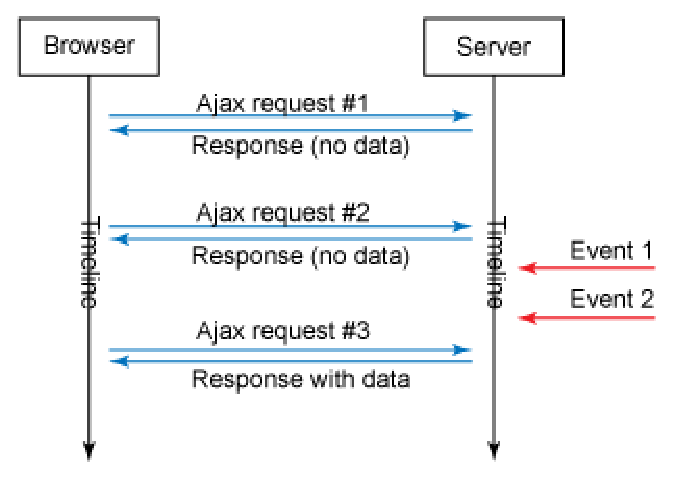
\includegraphics[scale=0.70]{figures/client_pull.eps}
    \caption{Client Pull Work Flow}
    \label{fig:client_pull}
\end{figure}
\begin{figure}[htb!]
    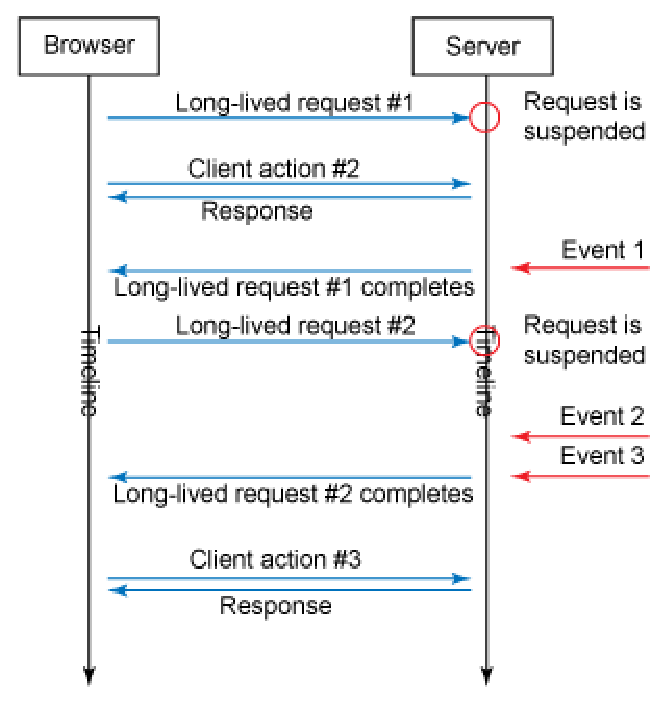
\includegraphics[scale=0.70]{figures/long_polling.eps}
    \caption{Long Polling Work Flow}
    \label{fig:long_polling}
\end{figure}

The down-side of long polling is that the server may have to deal with large
number of active connections between the clients and the servers. For example,
if you have one million users and, 10\% of them will be online. In this case,
the server should be able to hold at least 100,000 concurrent connections.

To address these problems, we present the event-based\cite{UnixBook}  long polling 
server PushUp that can provide long polling service with less resource cost.

As illustrated in Figure \ref{fig:sim_pushup}, the PushUp server lies in 
between of clients and web servers. It has two main responsibilities:
\begin{figure}[htb!]
\centering
    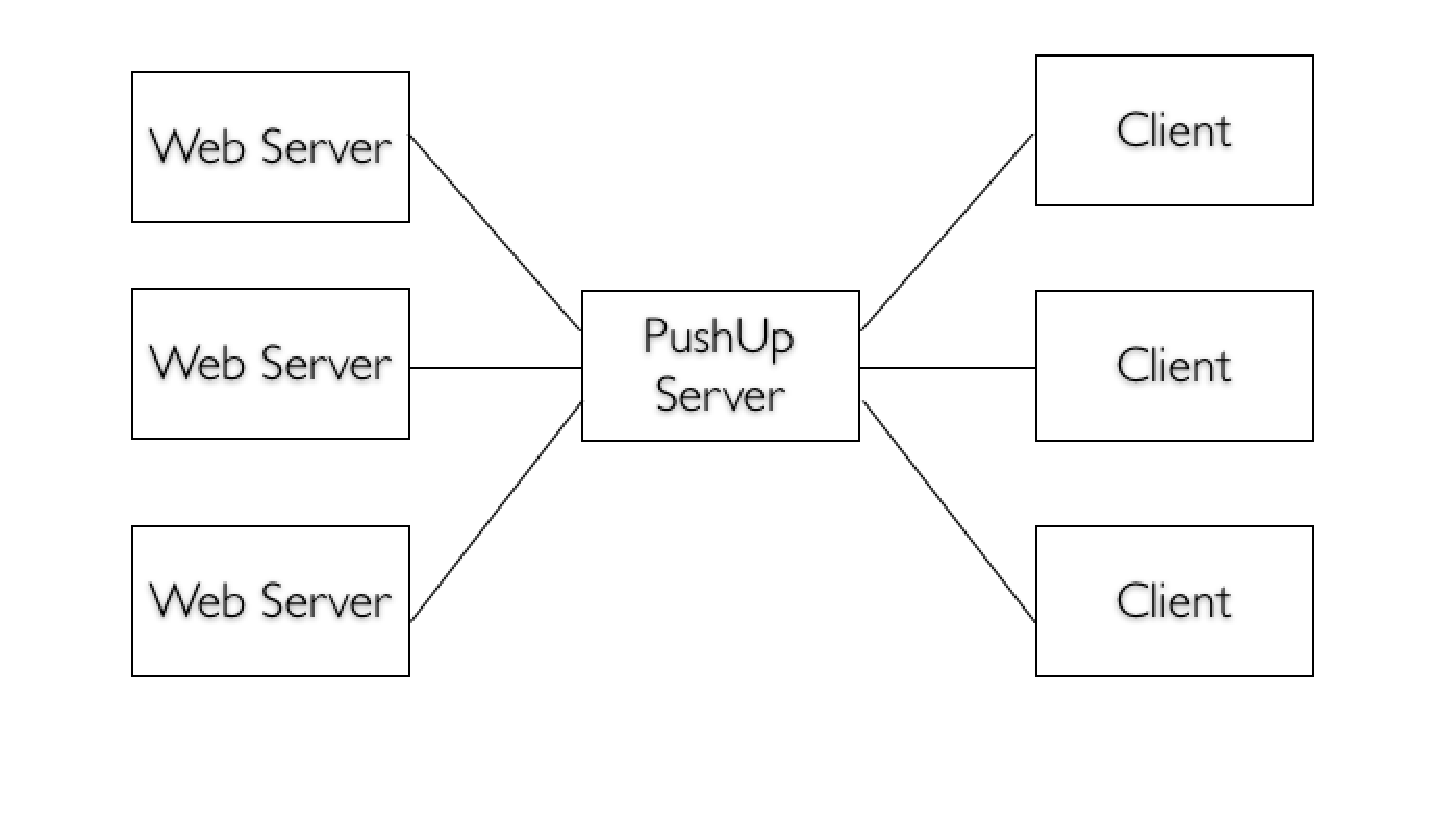
\includegraphics[scale=0.40]{figures/sim_pushup.eps}
    \caption{Simplified Architecture of the PushUp}
    \label{fig:sim_pushup}
\end{figure}

\begin {itemize}
\item {\bf An event-based reverse proxy}\cite{ReverseProxy} that retrieves 
resources on behalf of a client from one or more servers. We will cover
more on the details of reverse proxy in the following sections.
% When there are many 
% requests coming to the web server, the server needs to create many parallel 
% threads/processes and keep them running while client will close connection. 
% If client has slow connection, web server process will wait too long and 
% resource consumption will increase very fast. The reverse proxy can hide 
% the existence of the backend web server and 
% proxy can effectively solve the problem since 
\item {\bf A dedicated event-based message queue}\cite{PubSub} that can keep active 
connections with very low overhead. This message queue provides publication
interface for the web servers and the subscription interface for the clients.
\end {itemize}

